%You can delete all the comments after you have finished your document
%this sets up the defaults for the documents, 12pt font and A4 size. The article type sets this up as such as opposed to letter or memo.

%for the finer points LaTeX see https://en.wikibooks.org/wiki/LaTeX or http://tex.stackexchange.com/

\documentclass[12pt,a4paper]{article}
\usepackage{titlesec} %these are how we import packages, one helps set up footers and title layout
\usepackage{fancyhdr}

% !TEX TS-program = pdflatex
% !TEX encoding = UTF-8 Unicode
\usepackage[utf8]{inputenc} % set input encoding (not needed with XeLaTeX)

\usepackage{graphicx} % support the \includegraphics command and options

% \usepackage[parfill]{parskip} % Activate to begin paragraphs with an empty line rather than an indent

%%% PACKAGES
\usepackage{booktabs} % for much better looking tables
\usepackage{array} % for better arrays (eg matrices) in maths
\usepackage{graphicx}
\usepackage{paralist} % very flexible & customisable lists (eg. enumerate/itemize, etc.)
\usepackage{verbatim} % adds environment for commenting out blocks of text & for better verbatim
\usepackage{subfig} % make it possible to include more than one captioned figure/table in a single float
\usepackage{listings}
\usepackage[toc,page]{appendix}
% These packages are all incorporated in the memoir class to one degree or another...

%header and footer settings
\pagestyle{fancyplain}
\fancyhf{}
\renewcommand{\headrulewidth}{0.5pt}
\renewcommand{\footrulewidth}{0.5pt}
\setlength{\headheight}{15pt}
\fancyhead[L]{Mark Barton - 40204953}
\fancyhead[R]{Enhancing MonkeyPuzzle}
\fancyfoot[L]{}
\fancyfoot[C]{\thepage}

%set better section layout
\makeatletter
\renewcommand\subsection{\@startsection {subsection}{1}{2mm} % name, level, indent
                               {3pt plus 2pt minus 1pt} % before skip
                               {3pt plus 0pt} % after skip
                               {\normalfont\bfseries}}
\makeatother
\makeatletter
\renewcommand\section{\@startsection {section}{1}{0mm} % name, level, indent
                               {4pt plus 2pt minus 1pt} % before skip
                               {4pt plus 0pt} % after skip
                               {\bfseries}}
\makeatother


%this starts the document
\begin{document}

%you can import other documents into your main one, these layout the Title and Declarations on its own page.
%you might need to change these to \ if your on Microsoft Windows.
\newcommand{\HRule}{\rule{\linewidth}{0.5mm}}

\begin{titlepage}
	\begin{center}

	\HRule \\[0.4cm]
    	{\Large \bfseries Enhancing MonkeyPuzzle: Support for Analysing Web Resource\par}
	\vspace{0.2cm}
	\HRule \\[1.5cm]

	
    	\vspace{3cm}
	\begin{minipage}{0.4\textwidth}
	\begin{center} \large
        \emph{}\\
        	Mark Barton - 40204953
				
   	 \end{center}
    	\end{minipage}
	
	\vspace{2cm}
    	\begin{minipage}{1\textwidth}
    	\begin{center} \large
        
		Submitted in partial fulfilment of \\
		the requirements of Edinburgh Napier University \\
		for the Degree of \\
        	BEng (Hons) Software Engineering
    	\end{center}
    	\end{minipage}

    	\vfill

    	% Bottom of the page
	\begin{minipage}{1\textwidth}
    	\begin{center} \large
		School of Computing
    	\end{center}
    	\end{minipage}
	
	\vspace{1cm}
    	{\large \today}


	\end{center}
\end{titlepage}
%{\large Submitted in partial fulfilment of the requirements of Edinburgh Napier University for the Degree of }

\section*{Authorship Declaration}
\vspace{0.5cm}
\begin{flushleft}
I, Mark Allan Barton, confirm that this dissertation and the work presented in it are my own achievement.\newline

Where I have consulted the published work of others this is always clearly attributed;\newline

Where I have quoted from the work of others the source is always given. With the exception of such quotations this dissertation is entirely my own work;\newline

I have acknowledged all main sources of help; \newline

If my research follows on from previous work or is part of a larger collaborative research project I have made clear exactly what was done by others and what I have contributed myself;\newline

I have read and understand the penalties associated with Academic Misconduct.\newline

I also confirm that I have obtained informed consent from all people I have involved in the work in this dissertation following the School's ethical guidelines.\newline
\end{flushleft}

\begin{flushleft} \large
\emph{Signed: Mark Barton} \\
\end{flushleft}

\vspace{.5cm}

\begin{flushleft} \large
\emph{Date: 5th October 2018} \\
\end{flushleft}

\vspace{.5cm}

\begin{flushleft} \large
\emph{Matriculation no: 40204953}  \\
\end{flushleft}
\pagebreak

\section*{General Data Protection Regulation Declaration}
\vspace{0.5cm}
\begin{flushleft}
Under the General Data Protection Regulation (GDPR) (EU) 2016/679, the University cannot disclose your grade to an unauthorised person. However, other students benefit from studying dissertations that have their grades attached. \newline

\vspace{0.5cm}

Please sign your name below one of the options below to state your preference.\newline
\vspace{0.5cm}

The University may make this dissertation, with indicative grade, available to others.\newline
\vspace{0.5cm}

\emph Mark Barton. \newline
\vspace{2cm}


The University may make this dissertation available to others, but the grade may not be disclosed.\newline
\vspace{3cm}


The University may not make this dissertation available to others.\newline
\end{flushleft}



\pagebreak

%LaTeX let you define the abstract separately so it wont get sucked into the main document.
\begin{abstract}
% fill the abstract in here
\end{abstract}
\pagebreak

\tableofcontents % is generated for you
\newpage

\listoftables
%generated in same way as figures
\newpage

\listoffigures
%you may have captions such as equations, listings etc they should all appear as required
%these are done for you as long as you use \begin{figure}[placement settings] .. bla bla ... \end{figure}
\newpage

\section*{Acknowledgements}
\subsection*{}
	I would like to give a very special thanks to my parents for their support throughout my course, giving encouragement and advice when I most needed it. \newline
    
    I would also like to thank my girlfriend, Delaney, for putting up with the long nights spent on my computer researching and developing this project.\newline
    
    lastly, I would like to thank my Supervisor, Simon Wells, for giving me the idea for this project and helping me overcome the many challenges I have faced whilst completing my research.
\newpage




\section{Introduction}

MonkeyPuzzle is an Argument Analysis Web Application created by Simon Wells. The application gives one the ability to break down and analyse arguments based on the study of Critical Argumentation. A user can import text data into the editor panel of MonkeyPuzzle and manipulate said text in order to exhaustively reason the cause, rebuttal, and eventual conclusion of the argument. The current version of the web-app is in need of improvement. The editor window which allows users to interact with the argumentation data is possibly the most robust and well-made part of the entire project. However, other features such as the read-in and save features are still in their infancy. \newline

Improving MonkeyPuzzle looks to build upon the work that others have done in order to make MonkeyPuzzle more robust, user-friendly, and flexible with the addition of two new features; A new read in feature that allows a user to access data from websites and cite them in the editor window, and a cloud-save feature which will allow users to save their projects to the cloud for later retrieval.

\newpage

\subsection{Project Background}


My contribution to MonkeyPuzzle focuses on the addition of two new features to the program. The first is a new read-in feature which will allow a user to access data from a website of their choosing. This feature will be implemented using a web-proxy, a highly specialised program designed to access the internet via a virtual network. Traffic coming from a proxy is hidden, making it the perfect solution to bypass certain security features such as CORS (Cross-Origin Resource Sharing). \newline

The second is a new save feature for MonkeyPuzzle. The current version of the web app uses a unique file format known as "SADFACE" (a JSON based file format) in order to save a user's session. This file is saved locally on the user's device via download. This system is outdated by today's standards, instead the user will have the ability to save their work to the cloud using a cloud storage facility such as Google Drive or Dropbox.

\newpage


\subsection{Aims and Objectives}

Lorem ipsum dolor sit amet, consectetur adipiscing elit, sed do eiusmod tempor incididunt ut labore et dolore magna aliqua. Ut enim ad minim veniam, quis nostrud exercitation ullamco laboris nisi ut aliquip ex ea commodo consequat. Duis aute irure dolor in reprehenderit in voluptate velit esse cillum dolore eu fugiat nulla pariatur. Excepteur sint occaecat cupidatat non proident, sunt in culpa qui officia deserunt mollit anim id est laborum. Lorem ipsum dolor sit amet, consectetur dolore eu fugiat nulla pariatur. Excepteur sint occaecat cupidatat non proident, sunt in culpa qui officia deserunt mollit anim id est laborum. \newline

This is a sub sub section with a list of bullet points.
\begin{itemize}\itemsep1pt
	\item A working X, that will be used for this investigation.
	\item Investigation of current tools and their potential use during an investigation of X .
	\item Programming of X with related frameworks Y and Z.
	\item That is all.
	\item And also this part.
\end{itemize} 

Lorem ipsum dolor sit amet, consectetur adipiscing elit, sed do eiusmod tempor incididunt ut labore et dolore magna aliqua. Ut enim ad minim veniam, quis nostrud exercitation ullamco laboris nisi ut aliquip ex ea commodo consequat. Duis aute irure dolor in reprehenderit in voluptate velit esse cillum dolore eu fugiat nulla pariatur. Excepteur sint. \newline

occaecat cupidatat non proident, sunt in culpa qui officia deserunt mollit anim id est laborum. Lorem ipsum dolor sit amet, consectetur dolore eu fugiat nulla pariatur. Excepteur sint occaecat cupidatat non proident, sunt in culpa qui officia deserunt mollit anim id est laborum. 

\newpage


\subsection{Scope and Limitations}

\newpage


\subsection{Structure of Paper}


\newpage


\section{Literature Review}


\subsection{Overview}

\begin{figure}
\centering
    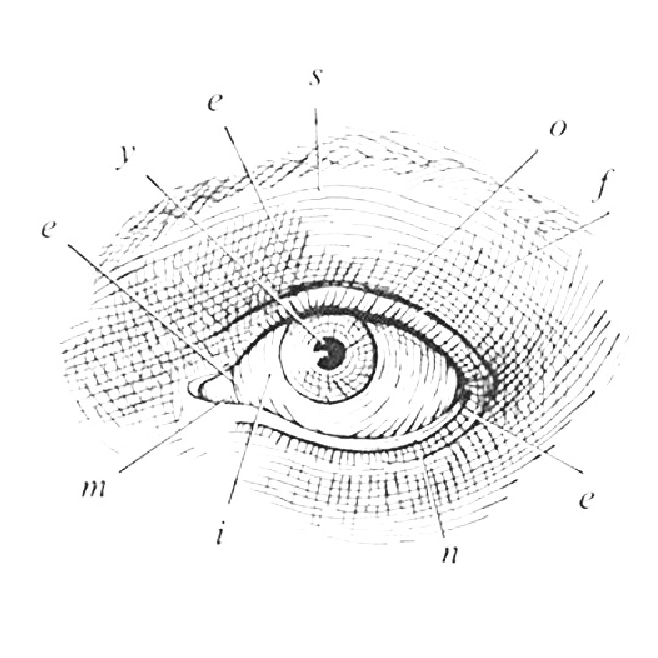
\includegraphics[scale = 0.5]{eye.eps}
    \caption{Image test}
    \label{fig:test}
\end{figure}



\subsection{Web Servers}

what is a web server
why do I need a web server

\subsubsection{Examples of Web Servers}

when are web servers needed
what are their purpose in terms of HTTP

\subsubsection{Proxies and VPNs}

what is a Proxy 
what is a VPN
what is the difference between them
which will I use

\subsubsection{Web Proxy}

what is a web proxy
what is it used for

\subsubsection{HTTP Proxy}

what is a HTTP Proxy
what is it used for

\subsubsection{Example Proxy}

demonstrate where proxies are used
explain why it is needed in this context

\newpage

\subsection{Website Security}

describe what web security is
explain why we need it

\subsubsection{Overview of Website Security}

When the internet was first conceived in (1970sss) the network was kept small and secure. It was used primarily to transfer data from one location to another without external interference. This initial version of the internet was created by (NAME) and was extensively used by the American government as a way to transfer intelligence and instructions across the country. It was more secure than radio (where the signal could be hijacked) and far more reliable than telephone (where interference could disrupt communication). 

The first version of the internet was used as a basic email system, and due to it being solely used by the government, it required no further security measures.

Fast-forward to (date), the first publicly available version of the internet was distributed world wide allowing users to interconnect with one another in a system we now refer to as the World Wide Web. This new form of internet used HTTP (Hypertext transfer protocol) to relay messages between servers (web hosts) and clients (home computers). This new type of protocol allowed users to transmit text messages and instructions to web servers which would in turn retrieve the files stored on the server and display the results on the user's web browser. 

There were no serious security measures in place for clients who accessed data off of a website, and as such, hackers were able to inject harmful lines of code into web servers. This would result in servers becoming overloaded with requests and eventually shutting down (DDoS attack), or infecting the visiting client's PC with a virus.

\subsubsection{SSL Certification}

explain what SSL Certificates are
explain why we need them

\subsubsection{AJAX and XMLHttpRequest}

describe what AJAX methods are
explain why XMLHttpRequest was used

note that this is now redundent with the implementation of CORS in (2013)

\subsubsection{The Cross-Origin Policy}

explain what the cross origin policy is
explain why it was implemented


\subsubsection{Cross-Origin Resource Sharing (CORS)}

explain how Cross origin resource sharing links with the project
explain what this means
explain how CORS works

\begin{figure}
\centering
    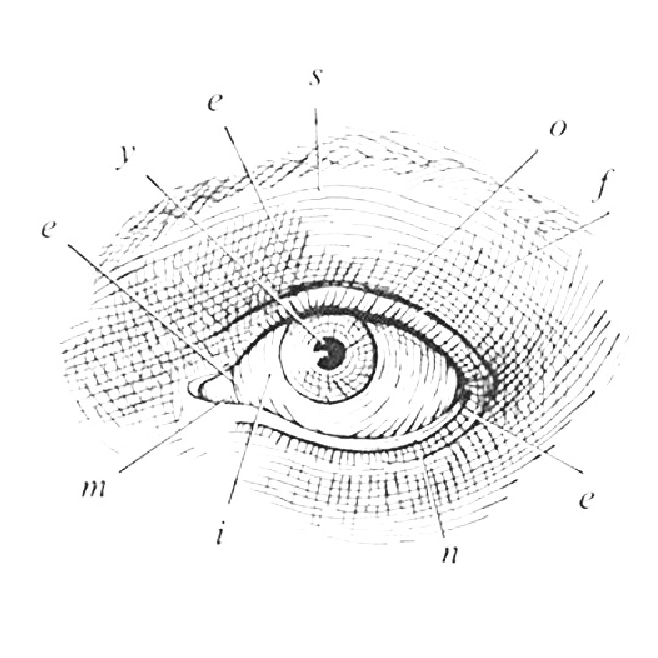
\includegraphics[scale = 0.5]{eye.eps}
    \caption{get picture of denied cross origin resource sharing from web console}
    \label{fig:CORS}
\end{figure}

\subsubsection{MIME Types}

explain what MIME types are
explain what they are used for
give and example of their use

\newpage


\subsection{Cloud Services}

explain what cloud services are
explain why I need them
give examples of cloud services

\subsubsection{Cloud Storage Capabilities}

describe how cloud storage works
demonstrate how it works (with figures)

\subsubsection{Real-life Examples of Cloud Storage}

give examples of real-life cloud storage usage

\subsubsection{Public, Private, and Hybrid Cloud Storage}

describe the difference between these types
describe which I will use

\newpage

\subsection{Conclusion}

inform what the fuck I am going to do

\newpage

\section{Technical Review}

\subsection{Overview}

introduce the technical review

\subsection{Python Web Proxy}

describe what a python web proxy is
explain why I need this

\subsubsection{Reasons for Python}

explain why i choose Python over something like NGINX
list the benifits of choosing Python

\subsubsection{Python Web Libraries}

inform about the Python Web Libraries
show methods I am going to use and list their arguments

\subsubsection{Web Server Example}

display a basic working version of the python web server including what it is doing for us.

\subsection{CORS}

description of the technical aspect of CORS

\subsubsection{The CORS Problem}

describe what issues are caused by CORS
detail how it gets in the way of what i am trying to achieve

\subsubsection{Requests Library}

brief description of what the Requests library does including specific commands I will use and its arguments

\subsubsection{MIME Requests}

Headers

Do Get

\subsubsection{GET Command}

brief description of the GET Command including its arguments

\subsubsection{HEAD Example}

how HEAD works

\subsection{Cloud Storage API}

brief description of what they are

\subsubsection{Dropbox API}

example

\subsubsection{Firebase Firestore}

what it is
how it works
implementing the API

example

\subsubsection{Amazon Web Services (AWS)}

what it is
how it works
implementing the API

example

\subsection{IDEs}

what IDEs I need to develop this

\subsubsection{Pycharm CE}

what it is
why I have chosen it over something like Wing IDE

\subsubsection{Brackets}
what it is
why I have chosen it over something like Sublime text

\subsubsection{Mozilla Firefox}

what it is
why I have chosen it over Chrome or Edge

\subsection{Version Control}

\subsubsection{Git}
why I have chosen Git over something like SVN

\subsubsection{Github}

Why i have chosen Github over Bitbucket

\subsection{Conclusion}

explain why I am doing what I am doing in regards to the technical aspect

\newpage

\section{Design}

\subsection{Overview}
how I am going to build this system
how I am going to implement this system
things I need to take into consideration

\subsection{Requirements Analysis}

\subsubsection{MoSCoW Priority Table}

\begin{center}
\begin{tabular}{ | m{4em} | m{24em}| } 
\hline
Priority & Item \\ [1pt]
\hline
Must Do & dsfdsfdsfsdfsf fsdflkdsfl n fldn djn lkj lhds lfhkj hsdlkjdsh flkjsadhbksdbnb kjsdhh sdahh fhfkj ha hsad f \\ 
\hline
Must Do & dsfadasdsdffsad sdfasdf dsfasdf \\ 
\hline
\end{tabular}
\end{center}


\subsubsection{Function Requirements Table}

\begin{center}
\begin{tabular}{ | m{4em} | m{24em}| } 
\hline
Priority & Item \\ [1pt]
\hline
Must Do & dsfdsfdsfsdfsf fsdflkdsfl n fldn djn lkj lhds lfhkj hsdlkjdsh flkjsadhbksdbnb kjsdhh sdahh fhfkj ha hsad f \\ 
\hline
Must Do & dsfadasdsdffsad sdfasdf dsfasdf \\ 
\hline
\end{tabular}
\end{center}


\subsubsection{Non-Functional Requirements Table}

\begin{center}
\begin{tabular}{ | m{4em} | m{24em}| } 
\hline
Priority & Item \\ [1pt]
\hline
Must Do & dsfdsfdsfsdfsf fsdflkdsfl n fldn djn lkj lhds lfhkj hsdlkjdsh flkjsadhbksdbnb kjsdhh sdahh fhfkj ha hsad f \\ 
\hline
Must Do & dsfadasdsdffsad sdfasdf dsfasdf \\ 
\hline
\end{tabular}
\end{center}

\newpage

\subsection{Web Proxy Design}

discuss how the web proxy will work. show diagrams of this
show how 

\subsubsection{Server Architecture}
how I run the server with python http server

\subsection{Bypassing CORS}

\subsection{Cloud Saving}

discuss how cloud saving is used in other systems
discuss how i will make it seamless and easy

\subsubsection{Integrating the API}

\subsection{Conclusion}

\newpage


\section {Implementation}

The project is split into three main sprints each lasting approximately two weeks each. The full sprint plan and sprint timeline can be viewed in Appendix B for further analysis. The first sprint focuses on the implementation of the Website resource panel; adding the new panel to MonkeyPuzzle, building the Proxy Script, displaying results in the panel, and giving users the ability to interact with the data within the editor panel. \newline

The second sprint focuses on the implementation of the cloud-save feature; implementing the Dropbox API, displaying the log-in dialogue, and saving/loading SADFace files to and from a Dropbox account. \newline

Lastly, the final sprint is dedicated to adding minor changes and improvements to the Web app including better positioning of elements, various tooltips to better help users navigate the web app, improved resizing of the resource panel, etc... \newline


\newpage

\subsection{Sprint 1 (Website Proxy)}

The first sprint commences on the 2nd of January. This sprint focuses on the development of the web resource panel. The panel is developed using JavaScript.

\subsubsection{Website Panel}

The current version of MonkeyPuzzle utilises a menu drawer known as the resource pane. Within this pane the user can add multiple resource panels for further analysis. The only resource type available currently is the text resource, allowing a user to import text files for later data manipulation. The new web resource panel will follow a similar design to the text resource panel as to improve general usability and User Experience Design.\newline

When new resources are added to the resource pane, a modal appears with a drop down list displaying all available resources. This modal has the id "resource\_type" which is used to help resourcepane.js script identify which type of resource is being created. By adding a second option called "web" to the list MonkeyPuzzle will be able to use this in order to populate the resource panel with the corresponding resource panel script. \newline.

a few new lines need to be added to the resourcepane.js in order to display a new web resource panel.\newline




The "File Name" text box is changed to "Website Address", allowing users to input a web address of their choosing before the proxy accesses and displays the results. Lastly, the "Content" text box is replaced with an iFrame in order to display the web-page requested by the user. This iFrame is made scaleable so that the user can expand and shrink the panel to their liking.

\begin{figure}
\centering
    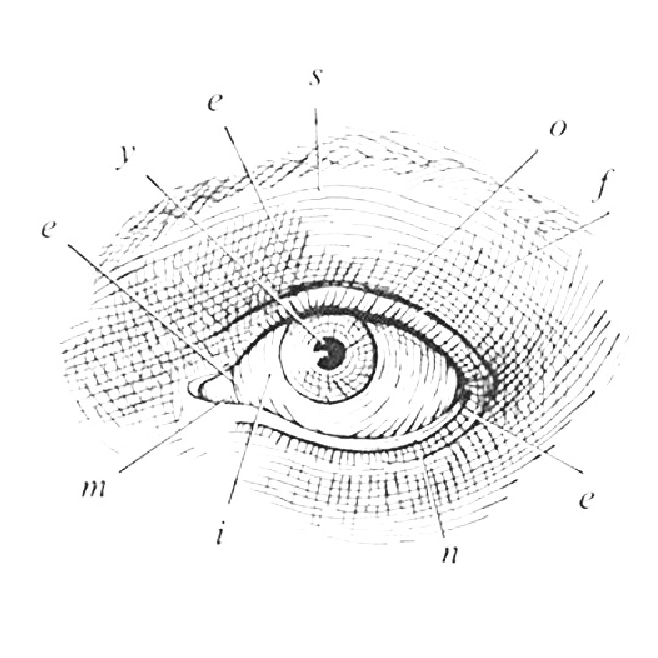
\includegraphics[scale = 0.5]{eye.eps}
    \caption{Web Resource Panel}
    \label{fig:Web Resource Panel}
\end{figure}


\subsubsection{Running Proxy on Server}

show web\_resource.py \newline

a virtual server was setup for me in the university, I connected to this using Cyberduck 6.8 (SSH).

\subsubsection{Interacting with Elements}

show atom code in resourcepanel\_web.js

\subsubsection{Saving State}



\subsection{Sprint 2 (Cloud Saving)}

\subsubsection{Integrating the API}



\subsection{Sprint 3 (Additional Features)}

\subsubsection{Resource Functions}

The text panel comes in three sections; a button control panel, a "File Name" text box, and a "Content" text box. The button control is made up of five functions.

\begin{itemize}\itemsep1pt
	\item Remove tab from the resource pane.
	\item Load text file.
	\item Save text file.
	\item Toggle editability of the content area.
	\item Add node from text selection.
\end{itemize}

These buttons are useful for the text resource panel, however, for the web resource panel these buttons are replaced with three new functions.

\begin{itemize}\itemsep1pt
	\item Previous website in history
	\item Next website in history.
	\item View website history.
\end{itemize}




add a website history list button to web panel

add hover tool tips to menu items in Resource panel

make the resource panel hide able.



\section{Testing}

\subsection{Overview}

describe what I am testing
outline the basis of tests

server based tests are done using a virtual server set up by Napier and accessing it using Cyberduck (SSH).

\subsection{Unit Testing}

\subsection{First Sprint Testing}

\subsubsection{Test Table}

\subsubsection{Test Results}

\subsection{Second Sprint Testing}

\subsubsection{Test Table}

\subsubsection{Test Results}

\subsection{Final Sprint Testing}

\subsubsection{Test Table}

\subsubsection{Test Results}

\subsection{Conclusion}

\newpage


\section{Evaluation}

\subsection{Evaluation of Goals}

\subsubsection{Proxy}

\subsubsection{Display}

\subsubsection{Cloud-Save}

\subsubsection{Conclusion}

\subsection{Evaluation of Project Management}

\subsubsection{Time Management}

\subsubsection{Project Controls}

\subsubsection{Version Control}

\subsubsection{Conclusion}

\subsection{Evaluation of Design}

\subsubsection{Software Architecture}

\subsubsection{UI/UX Design}

\subsection{Evaluation of Implementation}

\subsubsection{Proxy Method}

\subsubsection{Cross Origin Policy}

\subsection{Evaluation of Testing}

\subsection{Future Improvements}


\begin{thebibliography}{9}

\bibitem{lamport94}
  Leslie Lamport,
  \emph{\LaTeX: A Document Preparation System}.
  Addison Wesley, Massachusetts,
  2nd Edition,
  1994.

\end{thebibliography}
%example of References. See https://en.wikibooks.org/wiki/LaTeX/Bibliography_Management
%might be good to use a separate document for these so your main work is not one really long text file. 

%you can create this on a extra tex document just like the title or any other part of the document.
\newpage
\begin{appendices}
\section{Project Overview}
%insert IPO

\begin{subappendices}
\subsection{Example sub appendices}
...
\end{subappendices}

\section{Second Formal Review Output}
Insert a copy of the project review form you were given at the end of the review by the second marker

\section{Diary Sheets (or other project management evidence)}
Insert diary sheets here together with any project management plan you have

\section{Appendix 4 and following}
insert content here and for each of the other appendices, the title may be just on a page by itself, the pages of the appendices are not numbered, unless an included document such as a user manual or design document is itself pager numbered.
\end{appendices}

\end{document}
